    \chapter{Abstract Factory}
    \section{Intento}
    
    Fornisce un'interfaccia per creare famiglie di oggetti correlati o dipendenti senza specificarne le classi concrete, infatti il costruttore viene chiamato all'interno della factory.

    Nel progetto non useremo costruttori ma factory Method o Abstract Factory.


    %---
    \section{Struttura}

    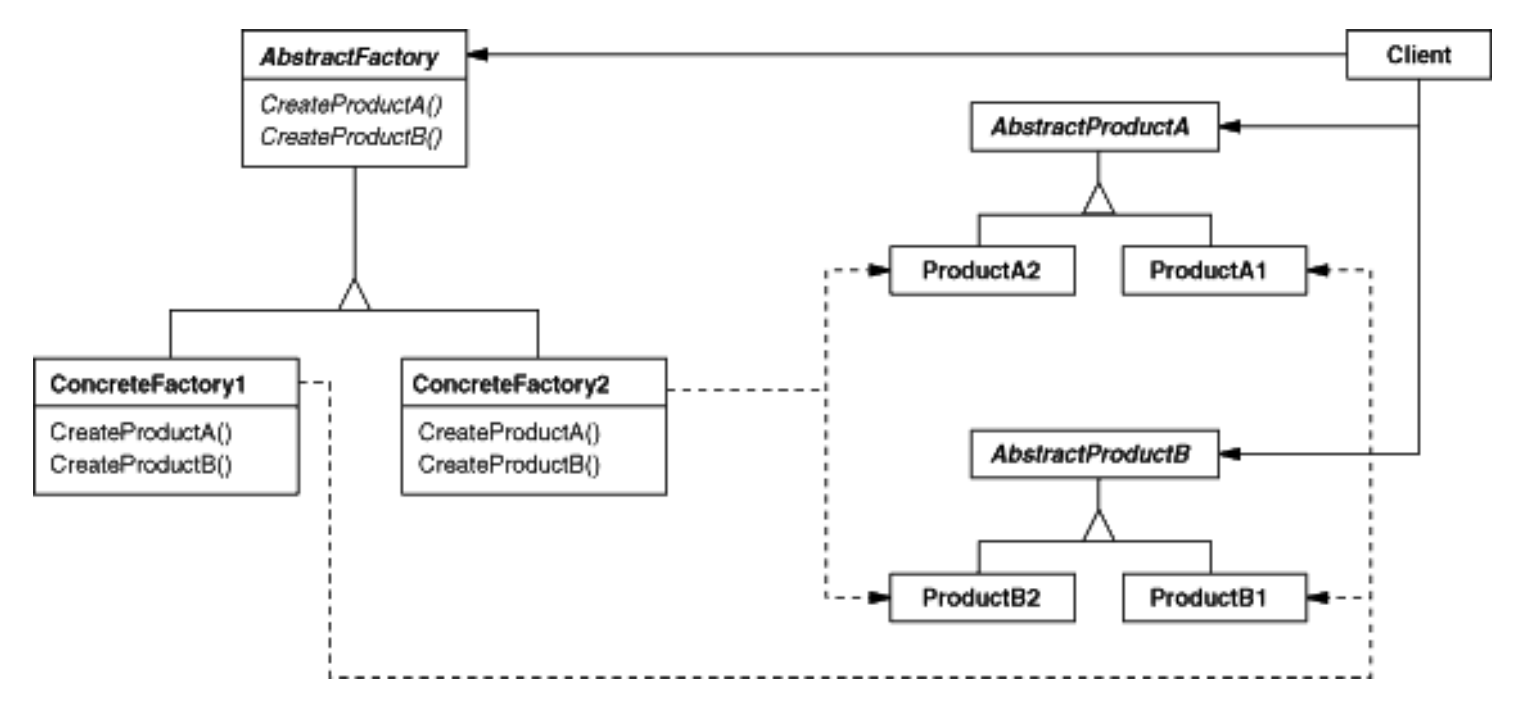
\includegraphics[width=\textwidth]{/Users/matt/Documents/GitHub/Design-Pattern-ITA/AbstractFactory/Structure1}


    %---
    \section{Implementazione}

    \subsection{Factory come Singleton.}
        Un'applicazione in genere richiede solo un'istanza di ConcreteFactory.

        Quindi di solito è meglio implementarlo come Singleton.

    \subsection{Creazione dei Product.}         
        AbstractFactory dichiara solo un'interfaccia per la creazione di prodotti. Spetta alle sottoclassi ConcreteProduct crearle effettivamente definendo un Factory Method per ciascun prodotto.
        
        Questa implementazione, quindi, richiede una nuova sottoclasse concreta per ogni famiglia di prodotti, anche se differiscono leggermente (se sono possibili molte famiglie di prodotti utilizzare il modello Prototype).
    

    %---
    \section{Esempio Java}
    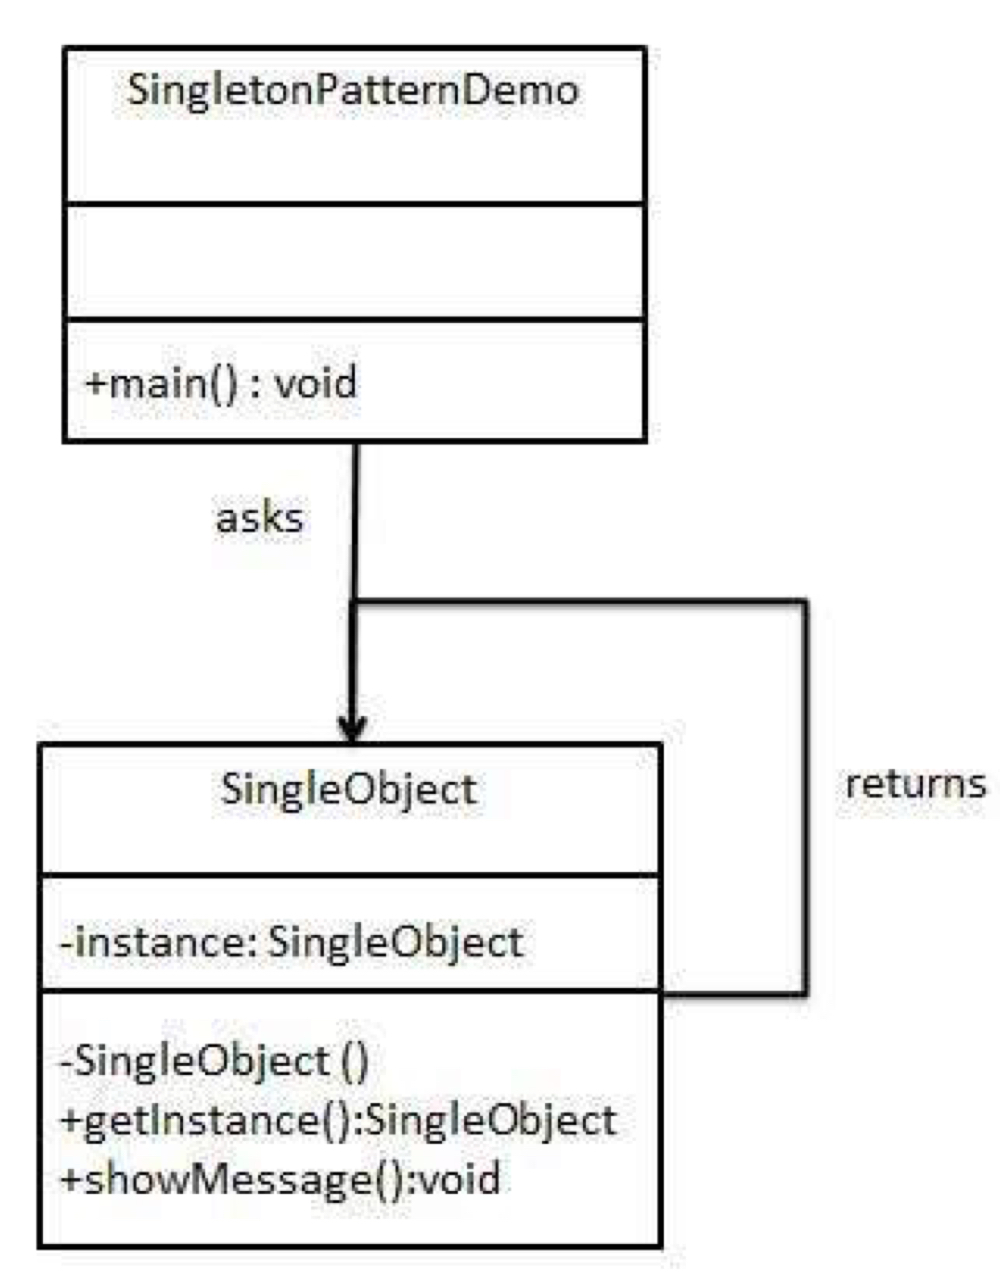
\includegraphics[width=\textwidth]{/Users/matt/Documents/GitHub/Design-Pattern-ITA/AbstractFactory/Example1}

    \subsection{FactoryProducer.java}
\begin{lstlisting}[language=java]
    public class FactoryProducer {
        public static AbstractFactory getFactory(boolean rounded) {
            if (rounded) {
                return new RoundedShapeFactor();
            } else {
                return new ShapeFactory();
            }
        }
    }
\end{lstlisting}

    \subsection{AbstractFactory.java}
\begin{lstlisting}[language=java]
    public abstract class AbstractFactory {
        abstract Shape getShape(String shapeType);
    }
\end{lstlisting}

    \subsection{ShapeFactory.java}
\begin{lstlisting}[language=java]
    public class ShapeFactory extends AbstractFactory {

        @Override
        public Shape getShape(String shapeType) {
            if (shapeType.equalsIgnoreCase("RECTANGLE")){
                return new Rectangle();
            } else if (shapeType.equalsIgnoreCase("SQUARE")) {
                return new Square();
            }
            return null;
        }
        
    }
\end{lstlisting}

    \subsection{RoundedShapeFactor.java}
\begin{lstlisting}[language=java]
    public class RoundedShapeFactor extends AbstractFactory {

        @Override
        public Shape getShape(String shapeType) {
            if (shapeType.equalsIgnoreCase("RECTANGLE")){
                return new RoundedRectangle();
            } else if (shapeType.equalsIgnoreCase("SQUARE")) {
                return new RoundedSquare();
            }
            return null;
        }
    }
\end{lstlisting}

    \subsection{Shape.java}
\begin{lstlisting}[language=java]
    public interface Shape {
        void draw();
    }
\end{lstlisting}

    \subsection{Rectangle.java}
\begin{lstlisting}[language=java]
    public class Rectangle implements Shape{

        @Override
        public void draw() {
            System.out.println("RETTANGOLO");
        }
        
    }
\end{lstlisting}

    \subsection{Square.java}
\begin{lstlisting}[language=java]
    public class Square implements Shape{

    @Override
    public void draw() {
        System.out.println("QUADRATO");
    }
    
}
\end{lstlisting}

    \subsection{RoundedRectangle.java}
\begin{lstlisting}[language=java]
    public class RoundedRectangle implements Shape{

        @Override
        public void draw() {
            System.out.println("RETTANGOLO ARROTONDATO");
        }
        
    }
\end{lstlisting}

    \subsection{RoundedSquare.java}
\begin{lstlisting}[language=java]
    public class RoundedSquare implements Shape{

        @Override
        public void draw() {
            System.out.println("QUADRATO ARROTONDATO");
        }
        
    }
\end{lstlisting}

    \subsection{main}
\begin{lstlisting}[language=java]
    public static void main(String[] args) {
    AbstractFactory shapeFactory = FactoryProducer.getFactory(false);

    Shape s1 = shapeFactory.getShape("rectangle");
    s1.draw();

    Shape s2 = shapeFactory.getShape("square");
    s2.draw();

    
    shapeFactory = FactoryProducer.getFactory(true);

    Shape s3 = shapeFactory.getShape("rectangle");
    s3.draw();

    Shape s4 = shapeFactory.getShape("square");
    s4.draw();
}
\end{lstlisting}
